\section{Resultat}
todo

\subsection{Parser} 
Parserns uppgift är att ta användarens indata och konvertera den till en datastruktur 
som är lättare att hantera internt. Denna datastruktur kallas AST (Abstract Syntax Tree). 
Haskellstandarden definerat upp en grammatik, ett antal regler som definerar hur korrekt Haskellkod ser ut och hur den ska tolkas.

För att parsa indatan använder vi ett bibliotek för att bygga parsers kallat JSParse \citep{jsparse}.
JSParse ger oss ett antal funktioner som vi använder för att definera grammatiken och konvetera den till vår interna struktur.

Som figur \ref{fig:parser_steg} visar, så består parsern av tre mindre parsers, den första är en parser som hittar kommentarer och tar bort dessa. 
Den andra identifierar Haskellkod som inte är kontextfri och gör om till kontextfri kod. Den tredje gör om den kontextfria koden till vår AST.

\begin{figure}[H]
    \begin{center}
        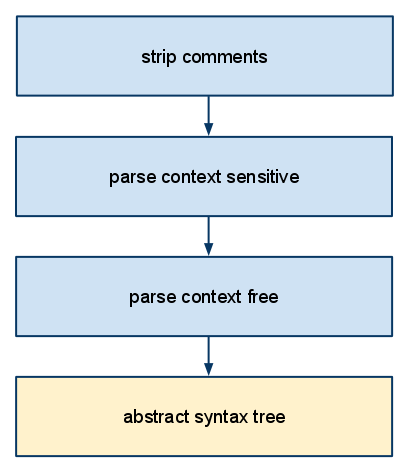
\includegraphics[width=.5\textwidth]{parser_1.png}
        \caption{Parserns olika steg}
        \label{fig:parser_steg} % Labels must come after caption!
    \end{center}
\end{figure}

Det var naturligt att dela upp parsern i tre olika steg. De tre olika stegen är skilda från varandra och vi kunde utveckla och testa dem individuellt.
Nedan följer ett exempel på parserns arbetssätt och de tre olika stegen:
\begin{lstlisting}
-- Kommentar
f x = case x of
    True -> False
    False -> True
\end{lstlisting}

Efter första steget:
\begin{lstlisting}
f x = case x of
    True -> False
    False -> True
\end{lstlisting}

Efter andra steget:
\begin{lstlisting}
f x = case x of {
    True -> False;
    False -> True
}
\end{lstlisting}

Efter det tredje steget är en AST genererad.
\begin{lstlisting}[language=javascript]
Function("f", Lambda("x", 
    Case(ast.VariableLookup("x"), [
        [PatternConstructor("True"), PatterConstructor("False")],
        [PatternConstructor("False"), PatterConstructor("True")],
    ])
))
\end{lstlisting}

\subsubsection{Steg 1}
Det första steget använder en parser som identifierar och tar bort kommentarer. 
Haskell har två olika kommentarsstiler, enkelradiga börjar med \emph{--} och slutar vid första radbytet och 
nästlade som kan gå över flera rader börjar med \emph{\{-} och slutar med \emph{-\}}.

\subsubsection{Steg 2}
Det andra steget delar upp koden i dess ord och symboler samtidigt som den dekoreras med indenteringsnivåer enligt en algoritm 
som är specifierad i Haskellstandarden. Därefter användads en annan algoritm från standarden för att sätta in måsvingar och semikolon på rätt platser. 
När de två algoritmerna är klara sätts koden ihop igen och skickas vidare till nästa steg.

En regel är att ett inre block inte får vara mindre indenterat än det omslutande blocket, exempelivs:
\begin{lstlisting}
case x of
    True -> ...
\end{lstlisting}
Här är \emph{True -> ...} ett inre block till \emph{case} och mer indenterat.

Ett annat exempel är:
\begin{lstlisting}
let x = 5 in x
\end{lstlisting}
Den korrekta översättningen är:
\begin{lstlisting}
let { x = 5 } in x
\end{lstlisting}
För att översätta detta korrekt kommer parsern ihåg den aktuella nästlingsnivån av "let"-uttryck och var deras repsektive "in"-uttryck befinner sig. 
Den avslutande måsvingen sätts in där ett matchande "in"-uttryck påträffas.

Ett exempel som inte översätts korrekt:
\begin{lstlisting}
[x | let x = 2]
\end{lstlisting}
Den korrekta översättningen är:
\begin{lstlisting}
[x | let { x = 2 }]
\end{lstlisting}
Men det blir:
\begin{lstlisting}
[ x | let { x = 2 ] }
\end{lstlisting}
Anledningen är att endast nästlingen av \emph{let} och \emph{in} sparas, men här finns inget \emph{in}.
För att lösa felet måste man hålla reda på antalet paranteser, måsvingar, hakparanteser och komman efter ett let-uttryck och när en symbol som gör det ogiltligt 
med en avslutande måsvinge påträffas sätts måsvingen in precis innan symbolen.

\subsubsection{Steg 3}
Det tredje steget är en parser för den kontextfria varianten av Haskell som den är definerad i standarden. 
Samtidigt som koden tolkas byggs en AST upp. Parsern består av en liten parser för varje grammatisk regel som är definerad i Haskellstandarden 
dessa parsers kombineras ihop för att bilda den slutgiltliga parsern. Det resulterar i ett träd av parsers, en parser för hela programmet som har flera mindre parsers under sig.

Exempel:
Definitionen i Haskellstandarden:
\begin{lstlisting}
gdrhs -> gd = exp [gdrhs]
rhs -> exp [where decls]
     | gdrhs [where decls]
\end{lstlisting}
Dess respektive parsers:
\begin{lstlisting}[language=javascript]
var gdrhs = gdrhs_action(
    repeat1(gdrhs_fix_list_action(sequence(ws(gd), 
                expectws('='), ws(exp)))));

var rhs = choice(
    decl_rhs_action(sequence(expect(ws('=')), ws(exp), 
         optional(sequence(expect(ws("where")), ws(decls))))),
     sequence(ws(gdrhs), optional(sequence(expect(ws("where")), 
         ws(decls))))
);
\end{lstlisting}

Parsern använder Haskell 2010's \citep{haskell2010} metod för att lösa företrädesreglerna för operator då denna metoden är enklare än den som är definerad i Haskell 98. 
Metoden fungerar så att den löser företrädesreglerna först efter ett uttryck har parsats till en lista med operatorer 
och uttryck, när en operator påträffas i listan slås dess företrädesnivå upp i en tabell och ett träd med 
operatorer och uttryck skapas. Sista används trädet för att generera en AST för uttrycken.

\subsubsection{JSParse}
Vi använder en modifierad version av JSParse där vi har korrigerat två fel och lagt till fler parsers. Felen vi korrigerade var i butnot-parsern och i choice-parserns cachefunktion. 
Choice-parsern cachade resultat från parsers som misslyckades och det cachade resultatet användes i senare parsers, 
vi löste det med en stackbaserad cache där cachen för en parser som misslyckas raderas.

Parsers som vi har lagt till:
\begin{enumerate}
    \item{\emph{repeatn}: en parser som upprepar en parser minst \emph{n} antal gånger}
    \item{\emph{expectws}: en parser som tillåter blanksteg och inte retunerar någon ast, är en kombination av JSParse inbyggda parsers \emph{expect} och \emph{whitespace}}
\end{enumerate}



\subsection{Interpretator}
Interprentatorns uppgift är att tolka det abstrakta syntaxträden. Under interprenteringen används flera datastrukturer vars uppgift och struktur anges här.

\subsubsection{Thunk}
En Thunk är en avstannad beräkning, en continuation. En Thunk består av en Env och en Expression.

\begin{lstlisting}
data Thunk = Closure Env Expression
\end{lstlisting}

Haskell måste använda sig av non-strict evaluation vilket innebär att en uträkning inte får köras ifall den inte behövs. När en uträkning körs så innebär det att den resulterar i flertalet Thunks för de delar av beräkningen som ännu inte behövs. När värdet av en Thunk behövs kommer den att tvingas till en WHNF eller en ny Thunk. Anledningen till detta är att vi på så sätt minskar användandet av rekursion vilket minskar risken att vi får ett runtime error.

\subsection{Weak Head Normal Form}
En WHNF är ett partiellt evaluerat uttryck. Uttrycket har blivit evaluerat så långt att vi är säkra på att det retunerar något typ av värde, alltså något som inte är undefined. Ofta innehåller en WHNF referenser till ännu icke evaluerade uttryck, om de inte gör det sägs uttrycket vara i Normal Form.

\begin{lstlisting}
data WeakHead 
    = Data Identifier [HeapPtr]
    | LambdaAbstraction Env Pattern Expression
    | DelayedApplication Env Int [Declaration] [HeapPtr]
    | Primitive
\end{lstlisting}

En Data är resultatet av att applicera en algebraisk datakonstruktor på dess argument. Argumenten ges som en lista av HeapPtrs, det vill säga en lista av evaluerade eller icke evaluerade uttryck. Exemplevis resulterar Just 1 i en Data med Identifiern Just och en HeapPtr till det icke evaluerade uttrycket 1.

En LambdaAbstraction är körningsrepresentationen av en lambdafunktion, en environment är bunden till lambdafunktionen.

En DelayedApplication är ett specialfall av en LambdaAbstraction. Vi avsockrar inte Haskells funktionsdeklerationener vilket innebär att pattern matchning sker även vid funktionsapplication och inte bara i Case satser. Detta betyder att vi måste samla alla argument till en funktion innan vi kan avgöra vilken Expression som skall användas. En vidare beskrivning finns i kapitlet Declaration.

En Primitiv är ett Javascript-värde, till exempel en integer eller en double.

\subsubsection{HeapPtr}
De flesta implementationer av Haskell använder sig av Lazy Evaluation, vilket innebär att en Thunk kommer att tvingas maximalt en gång. I vår implementation används HeapPtr som en wrapper runt en Thunk, när en HeapPtr dereferenceras kommer Thunken att tvingas till en WHNF och HeapPtr uppdateras att peka till denna. Eftersom att tvingandet av en Thunk kan resultera i en ny Thunk så tvingas thunken en loop tills vi får en WHNF.

\begin{lstlisting}
this.dereference = function() {
    if (this.weakHead == undefined) {
        // We'll drive the execution here instead of recursing 
        // in the force method
        var continuation = this.thunk;
        while (continuation instanceof interpreter.Thunk) {
            continuation = continuation.force();
        }
        this.weakHead = continuation;
        this.thunk = null;
     }
     return this.weakHead;
};
\end{lstlisting}

\subsubsection{Env}
Environmenten är en stack av javascript hashes, hasherna består av en bindning mellan en Identifier och antingen en HeapPtr eller ett (Pattern, HeapPtr) par.  Den andra bindingstypen är resultatet av en Variable deklaration där man måste utföra en pattern match för att avgöra vilken HeapPtr som hör till vilken Identifier. När man läser ut en identifier som är bunden enligt den andra typen av binding så kommer en pattern match att utföras och alla identifiers i patternet kommer att bindas om som den första type alternativt en pattern match fail inträffar och en exception genereras.

\begin{lstlisting}
Env {
    a => ([a, b, 2], [1,2,3])
    b => ([a, b, 2], [1,2,3])
}
Env.find(a)
Env {
    a => 1
    b => 2
}
\end{lstlisting}

\subsection{Abstrakt syntaxträd} 
AST:en representeras av javascript-object men dess strukturella uppbyggnad ges här av Haskell datadefinitioner.

\subsection{Declaration}
Den första datatypen av intresse är Declaration. En declaration representerar en namnbindning antigen i en moduls globala definitionsområde eller i en let eller where bindning.

\begin{lstlisting}
data Declaration 
    = Variable pattern Expression
    | Data Identifier [Constructor]
    | Function Identifier [Pattern] 
        (Either [(Guard, Expression)] Expression)
\end{lstlisting}

Variable är en bindning av typen p = e där p är en Pattern och e en Expression. En Variable kan därför binda flera olika symboler på en gång. Till exempel [1:a:b:[]] = [1,2,3].

Function är en representation av haskell sockrade funktionsdefinitioner. Det är möjligt att avsockra dessa till en Variable binding med hjälp av Lambda och Case [TODO referens] men vi har valt att införa en speciell representation av funktionsdefinitioner. Till skillnad från traditionella kompilatorer så avsockras Function aldrig utan håller samma form även under interpreteringen. Tanken bakom detta är att det skall vara lättare att se sammanhanget mellan datan under körning och källkoden vilket gör det lättare att knyta samman den statiska källkoden med den dynamiska körningsdatan.

En Data deklaration definierar en algebraisk datatyp med konstruktorerna definierade som nedan
data Constructor = Constructor Identifier Int
Värt att notera här är avsaknaden av typvariabler och -argument, detta kommer att åtgärdas när typchekaren är integrerad.

Under interprenteringen av en dekleration binds de namn (Identifiers) som definieras av deklarationen till envioromenten. Vilken typ av binding som används beror på typen av deklaration, en Variable deklaration ger en Identifier => (Pattern, Expression) bindning.

\subsection{Expression}
En Expression är ett haskelluttryck.

\begin{lstlisting}
data Expression 
    = Constant Value
    | Lambda Pattern Expression
    | Let [Declaration] Expression
    | Case Expression [(Pattern, Expression)]
    | VariableLookup Identifier
    | Do [DoNotation]
    | List [Expression]
    | ArithmeticSequence Expression (Maybe Expression) 
                                    (Maybe Expression)
    | Primitive JavascriptFunction
\end{lstlisting}

När en Expression evalueras under en environment är resultatet antingen en Thunk (continuation, closure) eller en WHNF. Evaluering av en Constant resulterar antigen i en Primitiv en en avsockring av konstanten. I interprentatorn så är konstanta nummer (1) egentligen en algegraisk datatype (I\# 1\#) och denna avsockring sker fört under körning. När en Lambda evalueras returneras en LambdaAbstraction med evaluerings environmenten bunden. En Let evalueras genom att binda dess Declarations till environmenten och returnera en Closure över den nya environmenten och Let Expressionen. En Case evalueras genom att den första Expressionen i tuple listan vars Pattern matchar evalueras under den environmenten som resulterar från pattern matchen.
\begin{lstlisting}
this.eval = function(env) {
    var expr = new interpreter.HeapPtr(
                   new interpreter.Closure(env, this.expr));
    for (var i in this.cases) {
        var newEnv = env.derive();
        if (this.cases[i][0].match(newEnv, expr)) {
            return this.cases[i][1].eval(newEnv);
        }
    }
    throw new Error("No matching clause");
};
\end{lstlisting}
Att evaluera en VariableLookup under en environment är det samma som att leta upp den Identifiern i environmenten.

Do, List och ArithmeticSequence är inte evaluerade direkt utan de är avsockrade och sedan evalueras det avsockrade uttrycket. Avsockringsreglerna ges i Haskell 98 standarden \citep{haskell98chap3}.

En Primitive är en wrapper runt en javascript funktion. Att evaluera en primitive är det samma som att evaluera funktionen med environmenten som argument.

\subsection{Pattern}
Vi har implementerat fem stycken olika pattern matches från Haskell.
\begin{lstlisting}
Pattern = Constructor Identifier [Pattern]
    | VariableBinding Identifier
    | Combined Identifier Pattern
    | ConstantPattern Value
    | Wildcard
\end{lstlisting}
Under en pattern match händer två saker. Dels så kontrolleras att uttrycket som matchas verkligen stämmer överens med patternet, dels så binds de variabler som definieras i patternet till environmenten. 

En VariableBinding matchar alla uttryck och binder uttrycket till identifiern. En Constructor matchar de uttryck vars WHNF är en Data med samma identifier (samt samma typ, detta enforcas dock av typcheckaren) och alla sub-patterns matchar Data argumenten. Combined är en sammanslagning av en VariableBinding och en annan Pattern, i källkod så har de formen \emph{v@p}. Combined matchar de uttryck som matchar dess Pattern och binder ett matchat uttryck till Identifiern. En ConstantPattern matchar de uttryck som är exakt lika med värdet. Till sist så matchar en Wildcard alla uttryck.


\subsection{Typcheckare} 
Typcheckarens uppgift är att analysera AST:n, inferera typerna på dess olika
beståndsdelar och avgöra om sättet på vilket de används och interagerar med
andra beståndsdelar är konsekvent. Om så inte är fallet sägs programmet ha
typfel.

\subsubsection{Haskells typsystem}
Jämfört med mer konventionella språk (C, C++, Java etc) skiljer sig Haskell
och övriga statiskt typade funktionella språk på flera sätt. I de senare
medges i många fall att programmeraren själv inte behöver ge explicita
typdeklarationer för variabler och funktioner. Istället arbetar typcheckaren
med en process där kriterier samlas in för varje enskild beståndsdel och
sedan utifrån detta försöker finna en så allmän typ som möjligt eller om
detta inte är möjligt; meddela programmeraren om typfel. Denna process
kallas typinferens.

Typinferens möjliggör även för polymorfiska typer vilket innebär att
typcheckaren alltid försöker hålla en typ så allmän som möjligt. Om
exempelvis en funktion inte är beroende av funktionalitet associerad med en
specifik typ hos något av sina argument kan data av alla typer användas som
argumentet.

Utöver polymorfiska typer stödjer Haskell typklasser som gör överlagring av
funktioner möjligt. Typklasser är väldigt centralt i Haskell och ändrar
typcheckarens arbetssätt markant jämfört med liknande språk.

\subsubsection{Typvariabler och subtitutioner}
För att kunna arbeta på en hög abstraktionsnivå har typcheckaren sin egen
interna representation av typer.

\begin{lstlisting}
data Type = TVar Id Kind
          | TAp Type Type
          | TCon Id Kind
          | TGen Int     
\end{lstlisting}

TVar representerar typvariabler, TAp representerar applicering av typer och
TCon representerar typkonstruktorer för konkreta typer. TGen representerar
generiska typer och kommer bara användas i samband med kvantifiering av
typer internt i 

För att veta om en typvariabel ska appliceras med andra typer eller om det
är en enkel typ (nullary type) används kinds där * representerar en enkel
typ och exempelvis * -> * och * -> ( * -> * ) representerar komplexare
typer som beror är beroende av andra typer. Ett exempel på en enkel typ är
Integer (*) medan typkonstruktorn för listor [] har kind * -> * .

\begin{lstlisting}
data Kind = Star
          | Kfun Star Star
\end{lstlisting}

Att konstruera en typ med den här notationen är enkelt. Typen [a] ->
Integer som är typen för standardfunktionen length i Haskell beskrivs med
\begin{lstlisting}
(TAp
  (TAp
    (TCon "(->)" (Kfun Star (Kfun Star Star)))
    (TAp
      (TCon "[]" (Kfun Star Star))
      (TVar "a" Star)))
  (TCon "Integer" Star))
\end{lstlisting}

Substitutioner är funktioner som mappar typvariabler till andra typer och
används av typcheckaren för att hålla typer uppdaterade efterhand som
typcheckaren får med information. Ofta vill man finna en substitution som gör
två typer ekvivalenta. Detta görs genom något som kallas unifiering.

\subsection{HIJi}

HIJi är ett program som ger användaren ett GHCi-liknande användargränssnitt till Haskelltolken direkt i webläsaren. 
HIJi tar indata genom att funktioner skrivs in i HIJi som sedan tolkas av parsern och i sin tur bygger upp det abstrakta syntaxträdet. Därefter evalueras uttrycket utav interpretern och resultatet blir synligt i HIJi.

HIJi har stöd för att ladda externa moduler. Det gör man genom att skriva :l \emph{namn-på-modul}. Man får då tillgång till alla de funktioner som är skrivna i den modulen. Modulerna måste vara placerade på servern som HIJi laddades ifrån. Modulerna kan ej laddas direkt från användarens hårddisk på grund utav att javascript av säkerhetsskäl ej har skriv och läsrättigheter av användarens filsystem. HIJi har även en förladdad modul, Prelude, som innehåller en delmängd av de funktioner som finns i GHCis motsvarighet. 

Den indata som användaren skriver till HIJi sparas i ett objekt för att hantera historiken. Man bläddrar i historiken med piltangenterna Upp och Ner. Hela historik-objektet sparas även i en kaka som ett JSON-objekt. Av detta skäl är det möjligt att få tillgång till historiken när man startar en ny session av webbläsaren.

\begin{figure}[H]
    \begin{center}
        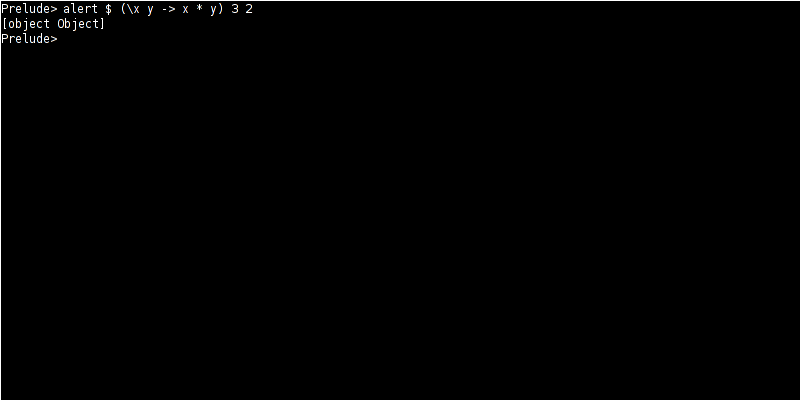
\includegraphics[width=1\textwidth]{hiji_screen3.png}
        \caption{HIJi användargränssnitt}
        \label{fig:hiji} % Labels must come after caption!
    \end{center}
\end{figure}

Figur \ref{fig:hiji} visar hur HIJi ser ut för användaren. De första raderna visar, precis som i GHCi, vilka moduler som för närvarande är laddade. I det här exemplet är den förladdade modulen Prelude laddad. Därefter följer en kommandotolk där användaren fritt kan skriva in egna funktioner. I figuren är en enkel lambda-funktion inskriven.

HIJi är skapat för att likna GHCi i så stor utsträckning som möjligt.
Genom att efterlikna GHCi kommer användare känna igen sig när de tar steget från HIJi till GHCi. Det blir för dem ett naturligt steg och kortar inlärningströskeln. Även för haskellprogrammerare som är vana användare utav GHCi blir det lättare att använda sig utav HIJi, de behöver inte fundera hur verktyget ska användas.
